\section{Le lièvre et la tortue (7 points + 3 bonus)}

\begin{center}
	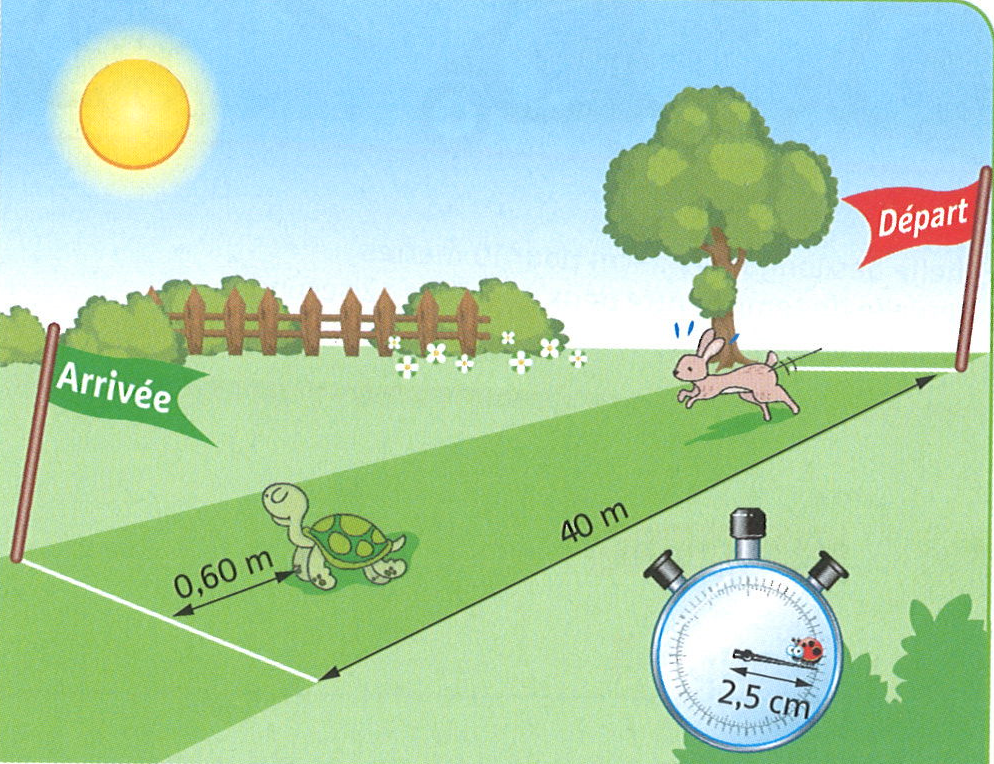
\includegraphics[scale=1.25]{lievre}
\end{center}

<<Rien ne sert de courir ; il faut partir à point>> est une maxime tirée de la fable <<le lièvre et la tortue>> de Jean de la Fontaine (1621 - 1695).\\


Après avoir fait la sieste sous un arbre à $\num{40.0}  m$  de la ligne d'arrivée, le lièvre se réveille et aperçoit la tortue qui le précède d'une distance $d = \num{39.4} m$. Elle file vers le succès dans cette ligne droite avec une vitesse de valeur constante $v_{tortue} = \num{0.2} m/s $.

Le lièvre se met alors à courir en accélérant jusqu'à atteindre une vitesse de valeur $v_{lievre} = \num{18.0} m/s$ et il s'y maintient.
\begin{questions}
	\question[1] Comment qualifie-t-on le mouvement de la tortue ?
	
%	\begin{parts}
%		\part[1] Comment qualifie-t-on le mouvement de la tortue ?
%		%\fillwithdottedlines{2cm}
%		%\part[1] Identifier et nommer les deux phases du  mouvement du lièvre.
%		%\fillwithdottedlines{2cm}
%		\part[2]Donner les trois caractéristiques de la vitesse de la tortue.
%		%\fillwithdottedlines{2cm}
%	\end{parts}

\vspace*{0.2cm}
	\question[2] Utiliser la formule de la vitesse
	
	\begin{parts}
		\part[1] Combien de temps faut-il à la tortue pour parcourir la distance qui la sépare de la ligne d'arrivée ?
		%\fillwithdottedlines{2cm}
		
		\part[1] Quelle distance peut parcourir le lièvre à sa vitesse maximale pendant cette même durée ?%maximale $d_{lievre}$ parcourrait le lièvre à sa vitesse maximale ?
		%\fillwithdottedlines{2cm}
	\end{parts}
\vspace*{0.2cm}
	\question[4] Lors de la phase d'accélération, on peut calculer la distance parcourue par le lièvre depuis l'arbre avec la formule suivante ($t$ est le temps que dure la phase d'accélération):
	
	\begin{equation*}
		distance = \num{4.5} \times t^2
	\end{equation*}

	\begin{parts}
		\part[2] On considère que cette accélération dure 2 secondes ; à quelle distance de l'arbre se trouve-t-il ?
		%\fillwithdottedlines{3cm}
		
		\part[1] A la fin de cette phase d'accélération, quelle distance lui reste-t-il à parcourir ?
		
		\part[1] Montrer alors qu'il a perdu la course.
		%\fillwithdottedlines{3cm}
	\end{parts}
\vspace*{0.2cm}

	\question[3] Une coccinelle, qui s'était endormie au bout de l'aiguille du chronomètre, fut entrainée dans son mouvement. \textbf{(Bonus)}
	
	\begin{parts}
		\part[1] Décrire la trajectoire de la coccinelle.
%		\fillwithdottedlines{2cm}
		
		\part[2] Calculer sa vitesse en cm/s, puis en m/s.
%		\fillwithdottedlines{3cm}
%		
%		\part[1] Tracer la flèche vitesse de la coccinelle en choisissant et précisant une échelle adaptée.
%		\makeemptybox{8cm}
%		
%		
%		
	\end{parts}
\end{questions}